\documentclass[oneside,12pt]{amsart}
\usepackage[english]{babel}
\usepackage{graphicx}
\usepackage{float}
\usepackage{mathtools}
\usepackage{amsfonts}
\usepackage{amssymb}
\usepackage{siunitx}
\usepackage{amsthm}
\usepackage{enumitem}
\usepackage{stmaryrd}
\usepackage{multirow}
\usepackage{caption}
\captionsetup[table]{position=bottom}
\usepackage[backend=bibtex,style=numeric]{biblatex}
\bibliography{Biblio}
\usepackage[a4paper, total={6in, 10in}]{geometry}
\graphicspath{{./}{}}% You can add the path for the images in the empty brackets 
\title{Capacitors: Wiring Parallel and in Series }
\author{Josh Goldfaden, Daniel Briseno}
\date{}
\newdimen\graph
\graph=4.2in
\newdimen\medgraph
\medgraph = 5.3in
\newdimen\smallgraph
\smallgraph = 3in
\newdimen\tinygraph
\tinygraph = 1.5in
\renewcommand{\arraystretch}{1.5}
\begin{document}
	\maketitle
	\section{Abstract}
	\indent In this lab, the effective capacitance of three capacitors, labeled A, B, and C, was studied when these provided capacitors were both wired in series as well as parallel to one another. Using a Digital Multi-meter, it was determined that the expected and actual capacitance (nF) of each arrangement had minimal discrepancies. In the second portion of this lab, a virtual capacitor constructed from two large, parallel conducting plates was studied. The change in voltage across each plate was analyzed as the plates were moved further apart from one another. It was found that as the distance between the plates increased, the voltage reading proportionally increased. 
	\section{Introduction}
	\indent A capacitor is a system of any two conductors that are separated by an insulator. Each of the conductors in a capacitor carry net excess charge that are equal in magnitude but are opposing charges. The capacitance, the ability of a system to store charge which is mathematically denoted as C, can be expressed as the following\cite{parallel}: 
	\begin{align*}
		C = \frac{Q}{V}
	\end{align*}
	where $ Q $ is the magnitude of excess charge possessed by each conductor and $V$ is the potential difference (potential) across both conductors.\\
	
	\indent Gauss' Law can be implemented to demonstrate that in an ideal parallel plate capacitor (a depiction of which is shown in Figure \ref{Ideal}), capacitance is directly related to the area $A$ of the plates. Further, Gauss' Law displays that the capacitance of this ideal parallel plate system is inversely related to the distance $d$ between the two plates \cite{parallel}: 
	\begin{align*}
		C = \frac{\kappa \epsilon _{0}A}{d}
	\end{align*}
	where  $\kappa$ is the dielectric constant that is dependent upon the properties of the insulator between the two conductive plates, and $\epsilon_0$ is the electric constant, often referred to as ''permittivity".\\
	\begin{figure}[H]
		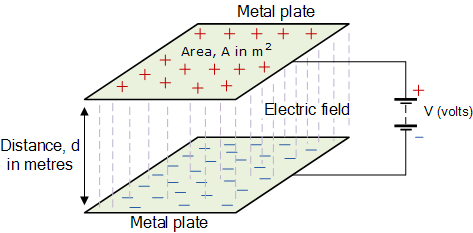
\includegraphics[width=\smallgraph,scale=0.01]{IdealCapacitor.png}
		%h (here) - same location
		%t (top) - top of page
		%b (bottom) - bottom of page
		%p (page) - on an extra page5
		%! (override) - will force the specified location
		\caption{Ideal plate capacitor. Photo Credit \cite{ideal}.}
		\label{Ideal}
	\end{figure}

	\indent We often connect capacitors to each other in series and in parallel. A depiction of capacitors in parallel can be seen in Figure \ref{Parallel}. In this case we know that the voltage across the two capacitors is equal\cite{cap} and thus we can derive :
	\begin{align*}
	C_{total} &= \frac{Q_{total}}{V} \\
	&=\frac{Q_1+Q_2}{V}\\
	&= \frac{Q_1}{V} + \frac{Q_2}{V}\\
	&= C_1 + C_2
	\end{align*}
	 
	\begin{figure}[h]
		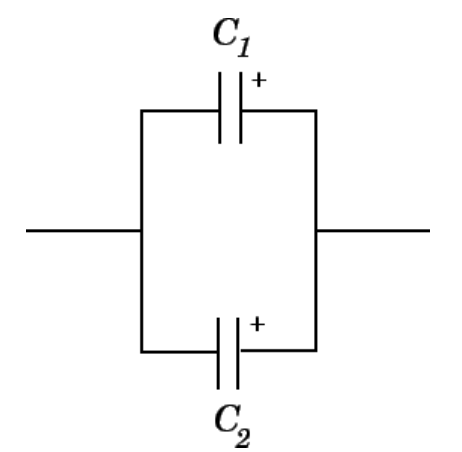
\includegraphics[width=\smallgraph,scale=0.01]{Parallel.png}
		%h (here) - same location
		%t (top) - top of page
		%b (bottom) - bottom of page
		%p (page) - on an extra page5
		%! (override) - will force the specified location
		\caption{Capacitors in parallel. Photo credit \cite{cap}}
		\label{Parallel}
	\end{figure}
\begin{figure}[h]
	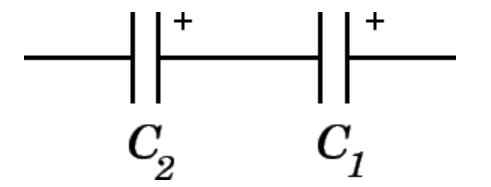
\includegraphics[width=\smallgraph,scale=0.01]{Series.png}
	%h (here) - same location
	%t (top) - top of page
	%b (bottom) - bottom of page
	%p (page) - on an extra page5
	%! (override) - will force the specified location
	\caption{Capacitors in series. Photo credit \cite{cap}}
	\label{Series}
\end{figure}

	
	\indent Figure \ref{Series} shows two capacitors connected in series. In this case we know that the excess charge $Q$ across both capacitors must be equal \cite{cap}, and we similarly compute:\\
	\begin{align*}
		\frac{1}{C_{total}} &= \frac{V}{Q}\\
		&= \frac{V_1 + V_2}{Q}\\
		&= \frac{V_1}{Q} + \frac{V_2}{Q}\\
		&= \frac{1}{C_1} + \frac{1}{C_2}
	\end{align*}


	\indent In summary, we can have the following four relations \cite{cap}\cite{parallel}:
	\begin{align}
	&\text{Definition of capacitance} &&	C = \frac{Q}{V}\\
	&\text{For an ideal capacitor} &&C = \frac{\kappa \epsilon _{0}A}{d}\\
	&\text{For capacitors in parallel} &&C_{total} = C_1 + C_2\\
	&\text{For capacitors in series} && \frac{1}{C_{total}} = \frac{1}{C_1}+\frac{1}{C_2}
	\end{align}
	
	\section{Experimental confirmation of equations 3 and 4}
	\indent In this section of the experiment we seek to gain empirical confirmation of equations (3) and (4) derived in the introduction.\\
	
	\indent In order to do this, we measured the capacitance of three capacitors A,B, and C. The results of these measurements can be seen in Table \ref{abc} 

	\begin{table}[h]
		\begin{tabular}{ |c|c|}
			\hline
			Capacitor & Measured Capacitance (nF)\\
			\hline
			A&105.8\\
			B&99.9\\
			C&121.1\\
			\hline
		\end{tabular}
		\caption{Capacitance of capacitors A,B, and C.}
		\label{abc}
	\end{table}

	\indent After taking these measurements, we used equation (3) predicted the capacitance of all parallel circuits we could make using the three capacitors, then we built the circuits and measured the actual capacitance. This process was repeated for circuits in series with equation (4), and the results are seen in Tables \ref{inParallel} and \ref{inSeries}, respectively. 
	\begin{table}[h]
		\begin{tabular}{ |c|c|c|c|}
			\hline
			Capacitors & Theoretical Capacitance(nF)& Measured Capacitance(nF) &\% Error\\
			\hline
			A and B	&205.7&205&0.341\\
			A and C&226.9 & 226&0.398\\
			B and C&221&220&0.455\\
			A, B and C&326.8&327&0.0612\\
			\hline
		\end{tabular}
		\caption{Capacitance of A,B, and C connected in parallel.}
		\label{inParallel}
	\end{table}

\begin{table}[h]
	\begin{tabular}{ |c|c|c|c|}
		\hline
		Capacitor & Theoretical Capacitance(nF)& Measured Capacitance(nF) &\% Error\\
		\hline
		A and B&51.4&51.2&0.391\\
		A and C&56.5&56.5&0\\
		B and C&54.7&54.4&0.552\\
		A, B and C&36.1&35.9&0.557\\
		\hline
	\end{tabular}
	\caption{Capacitance of A,B, and C connected in series.}
	\label{inSeries}
\end{table}
	
	As expected, our predictions are very close to our measured values, with a maximum error of 0.455\% for the parallel condition, and 0.557\% for the series condition. With such small errors, we can clearly say that we have strong evidence in favor of equations (3) and (4) and that our small errors are likely due to measurement inaccuracies. 

	
\section{Parallel Plate Capacitor: Potential Spacing vs. Spacing}
	In this part of the experiment, we wanted to study how a capacitor constructed from two large, parallel metal plates behaved as the distance between these plates changed. Specifically, we wanted to study how the voltage spread across each plate changed as the plates were moved further apart. This was achieved using a virtual lab.\\
	
	\indent We worked with the Logger Pro file, $<$SensorDataSet.cmbl$>$, which has the “movie” $<$CapacitorV\_vs\_d.mov$>$ integrated with it. This file was used to track and plot the voltage across one plate over an increasing distance. The data collected from the video is shown in Table \ref{Volt} and Figure \ref{VvD}.\\
	
	\begin{table}[h]
		\begin{tabular}{|c|c|c|}
			\hline
			Rotations (\# of turns) & Distance Between Plates (mm) & Voltage Readings (V)\\
			\hline
			0.0&0&0\\
			0.5&0.625&13.41\\
			1.0 &1.25&24.76\\
			1.5 &1.875&34.86\\
			2.0&2.5&44.13\\
			\hline
		\end{tabular}
		\caption{Measured plate voltage at various plate separation distances.} 
		\label{Volt}
	\end{table}

\begin{figure}[h]
	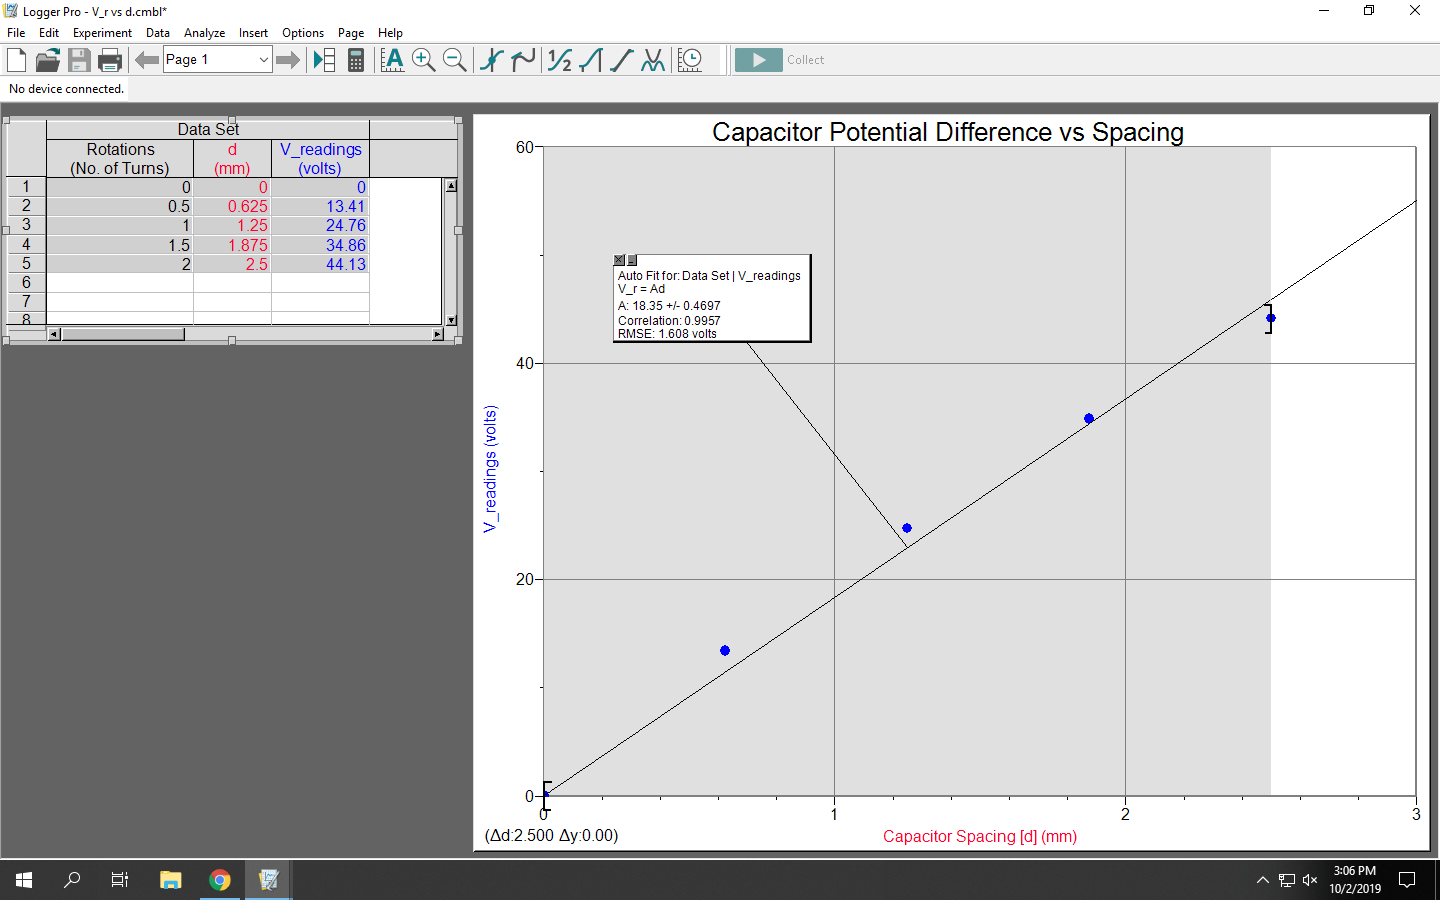
\includegraphics[width=\medgraph,scale=0.01]{VoltvDistance.png}
	%h (here) - same location
	%t (top) - top of page
	%b (bottom) - bottom of page
	%p (page) - on an extra page5
	%! (override) - will force the specified location
	\caption{Measured plate voltage vs plate separation.}
	\label{VvD}
\end{figure}

	\indent Recall from equations (1) and (2) that in a perfect capacitor, we have 
	\begin{align*}
	C = \frac{Q}{V} =  \frac{\kappa \epsilon _{0}A}{d}\\
	\end{align*}
	which implies
	
	\begin{align}
	V = d\frac{Q}{\kappa\epsilon_0A}
	\end{align}
	 where $Q$ is the excess charge on the conductor, A is the area of the capacitor, $d$ is the spacing between the capacitor plates and $\epsilon_0$ is the electric constant. We would expect that if $Q$ and $A$ are held constant, the voltage across the plates would be proportional to the distance between them.\\
	 
	 \indent In Figure \ref{VvD}, we see that $V$ is nearly proportional to $d$. Therefore, we can approximately model the behavior of the two plates in the video with that of an ideal capacitor. This allows us to use equation (5) to find the excess charge on the plates.\\
	 
	 \indent We are given that the diameter of each plate is $\approx 25.59$cm. So the area $A$ of each plate is $\pi(0.2559\times0.5\text{m})^2\approx 0.05143\text{m}^2$. Additionally, we are given that $\kappa \approx 1$, and we can see that when $d = 1.25$mm, $V \approx 25$V, so we can calculate:
	 
	 \begin{align*}
	 	Q&\approx \frac{V\epsilon_0A}{d}\\
	 	&\approx \frac{25 (8.85\times 10^{-12})0.05143}{1.25\times 10^-3}\text{C}\\
	 	Q&\approx 9.1\text{nC}	 	
	 \end{align*}
	 
	 \indent We end this section with a discussion of the differences between the behavior of the two plates and an ideal capcacitor. Although we can approximate the voltage across the two plates by using an ideal capacitor model reasonably well, a quick look at Figure \ref{VvD} shows that we cannot \textit{exactly} predict the values of $V$. In particular, we see that the first two points are nearly collinear with each other and the origin, while the last two are not as collinear with the initial points and show a weaker voltage than would have been expected if the linear relationship between the first two points had persisted. This indicates that we see behavior very similar to an ideal capacitor when $d$ is very small, but as $d$ increases the voltage no longer follows the predictions of an ideal capacitor model.\\
	 
	 \indent This is not a surprise, since the linear increase in voltage relies on the uniformity of the electric field. A truly uniform electric field can only be generated by disks of \textit{infinite} radius $R$. Obviously, this can not be the case in any laboratory setting, but when $d<<R$, the electric field will act very similarly to that of infinte charged plates.
	 
	 \section{Conclusion}
	 In the first section of this lab, we experimentally confirmed equations (3) and (4) by measuring the capacitance of capacitors in parallel and in series, and comparing these values to the values predicted by equations (3) and (4), respectivley. We found that we were able to predict capacitance remarkably well, with a maximum \% Error of 0.557\% across all trials.\\
	 
	 \indent In the second part of the lab, we investigated the behavior of two charged plates placed a various distances from each other (but always facing each other). We found that when the distance $d$ between the plates was small, the capacitance of the two plates was accuratley modeled by an ideal parallel-plate capacitor. By using this model, we found that the excess charge on the plates was $Q\approx 9.1$nC. Finally we ended the section by noting that the parallel plates only acted as an ideal capacitor when $d$ was small, and the voltage began rising slower than the linear model predicted for $d>1.5$ . We speculated that this was due to the electric field not being truly unifom, especially for $d$ large.
	
\newpage
\printbibliography
	 
	
\end{document}